\documentclass[aspectratio=169]{beamer}

\usepackage[utf8]{inputenc}
\usepackage{tikz}
\usetikzlibrary{positioning, arrows.meta, decorations.pathreplacing, calligraphy}
\usepackage{booktabs}
\usepackage{colortbl}
\usepackage{multirow}
\usepackage{array}

\usefonttheme{professionalfonts}

% Theme
\usetheme{Madrid}
\definecolor{ucdgreen}{RGB}{0, 102, 51}
\definecolor{availgreen}{RGB}{0, 153, 102}
\definecolor{derivblue}{RGB}{100, 160, 210}
\definecolor{partialgreen}{RGB}{0, 153, 102}
\definecolor{unavailgray}{RGB}{180, 180, 180}
\definecolor{nextfill}{RGB}{255, 240, 200}
\definecolor{gapred}{RGB}{180, 50, 50}
\definecolor{vennblue}{RGB}{70, 130, 180}
\definecolor{vennorange}{RGB}{210, 140, 50}
\usecolortheme[named=ucdgreen]{structure}
\setbeamertemplate{navigation symbols}{}

\title[Research Studies Panel]{Research Studies Panel}
\author[Lainey Ward]{Lainey Ward}
\institute[]{}
\date{}

\begin{document}

% --------------------------------------------------
% BACKUP: Dataset overview
% --------------------------------------------------
% USE: If panel asks "what data are you using?"
%      or "where does the data come from?"
% --------------------------------------------------
\begin{frame}{Dataset Overview}

    \centering
    \vspace{-0.3em}

    {\footnotesize\textbf{Forecast systems}}
    \vspace{0.3em}

    \footnotesize
    \renewcommand{\arraystretch}{1.3}
    \begin{tabular}{l l l l l l l}
    \toprule
    \textbf{System} & \textbf{Source} & \textbf{IFS cycle} & \textbf{Grid} & \textbf{Members} & \textbf{Reforecast period} & \textbf{Lead range} \\
    \midrule
    Seasonal (SEAS5)       & MARS API & Cy43r1 & 0.28\textdegree{} & 25 & 1981--2016 & 215 days \\
    Subseasonal (EEFH)     & MARS API & Cy49r1 & 0.28\textdegree{} & 11 & 2005--2024 & 46 days  \\
    \bottomrule
    \end{tabular}

    \vspace{0.8em}

    {\footnotesize\textbf{Reference datasets}}
    \vspace{0.3em}

    \footnotesize
    \renewcommand{\arraystretch}{1.3}
    \begin{tabular}{l l l l}
    \toprule
    \textbf{Dataset} & \textbf{Source} & \textbf{Grid} & \textbf{Coverage} \\
    \midrule
    ERA5-Land     & MARS API              & 0.1\textdegree{} & 1950--present \\
    Met \'Eireann & Met \'Eireann archive & Station          & 1945--present (varies by station) \\
    \bottomrule
    \end{tabular}

    \vspace{0.8em}
    \scriptsize
    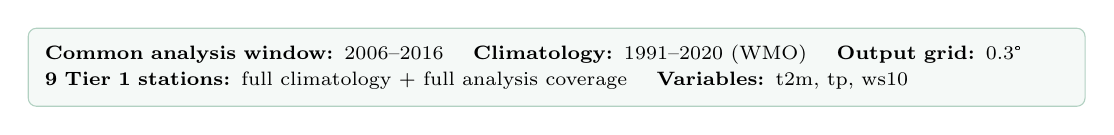
\begin{tikzpicture}
        \node[draw=ucdgreen!30, rounded corners=3pt, fill=ucdgreen!4,
              text width=13cm, align=left, font=\scriptsize, inner sep=6pt] {
            \textbf{Common analysis window:} 2006--2016 \quad
            \textbf{Climatology:} 1991--2020 (WMO) \quad
            \textbf{Output grid:} 0.3\textdegree{} \\[0.2em]
            \textbf{9 Tier~1 stations:} full climatology + full analysis coverage \quad
            \textbf{Variables:} t2m, tp, ws10
        };
    \end{tikzpicture}

\end{frame}

% --------------------------------------------------
% BACKUP: EEFH vs SEAS5 system comparison
% --------------------------------------------------
% USE: If panel asks "what's the difference between
%      the two systems?" or "why compare them?"
% --------------------------------------------------
\begin{frame}{Subseasonal vs Seasonal: System Comparison}

    \centering
    \vspace{-0.3em}

    \footnotesize
    \renewcommand{\arraystretch}{1.4}
    \begin{tabular}{l c c}
    \toprule
     & \textbf{Subseasonal (EEFH)} & \textbf{Seasonal (SEAS5)} \\
    \midrule
    IFS cycle            & Cy49r1 (2024)       & Cy43r1 (2016) \\
    Grid type            & Cubic octahedral     & Reduced Gaussian \\
    Resolution           & $\sim$32 km (TCo319) & $\sim$36 km (T319) \\
    Vertical levels      & 137                  & 91 \\
    Stochastic physics   & SPP (27 parameters)  & SPPT3 + SKEB \\
    Ozone--radiation     & Fully interactive    & Climatological \\
    Reforecast members   & 11                   & 25 \\
    Real-time members    & 101                  & 51 \\
    Init frequency       & Every odd day        & 1st of month \\
    Reforecast period    & Prior 20 yr (rolling) & 1981--2016 (fixed) \\
    Lead range           & 46 days              & 215 days \\
    Atm.\ initial conds  & ERA5                 & ERA-Interim \\
    \bottomrule
    \end{tabular}

    \vspace{0.8em}
    \scriptsize
    
\begin{tikzpicture}
        \node[draw=ucdgreen!30, rounded corners=3pt, fill=ucdgreen!4,
              text width=12cm, align=left, font=\scriptsize, inner sep=6pt] {
            \textbf{Matched comparison:} 2006--2016, 1st-of-month inits, 0.3\textdegree{} grid over Ireland. \\
            Differences then reflect \textbf{model physics and ensemble size}, not data coverage.
        };
    \end{tikzpicture}

\end{frame}

% --------------------------------------------------
% BACKUP: Terminology map
% --------------------------------------------------
% USE: If panel asks "what does the existing literature
%      look like?", "how fragmented is the field?", or
%      "why is there no standard definition?"
% --------------------------------------------------
\begin{frame}{How Do You Detect These Events?}

    \begin{columns}[c, totalwidth=\textwidth]

        \begin{column}{0.75\textwidth}
            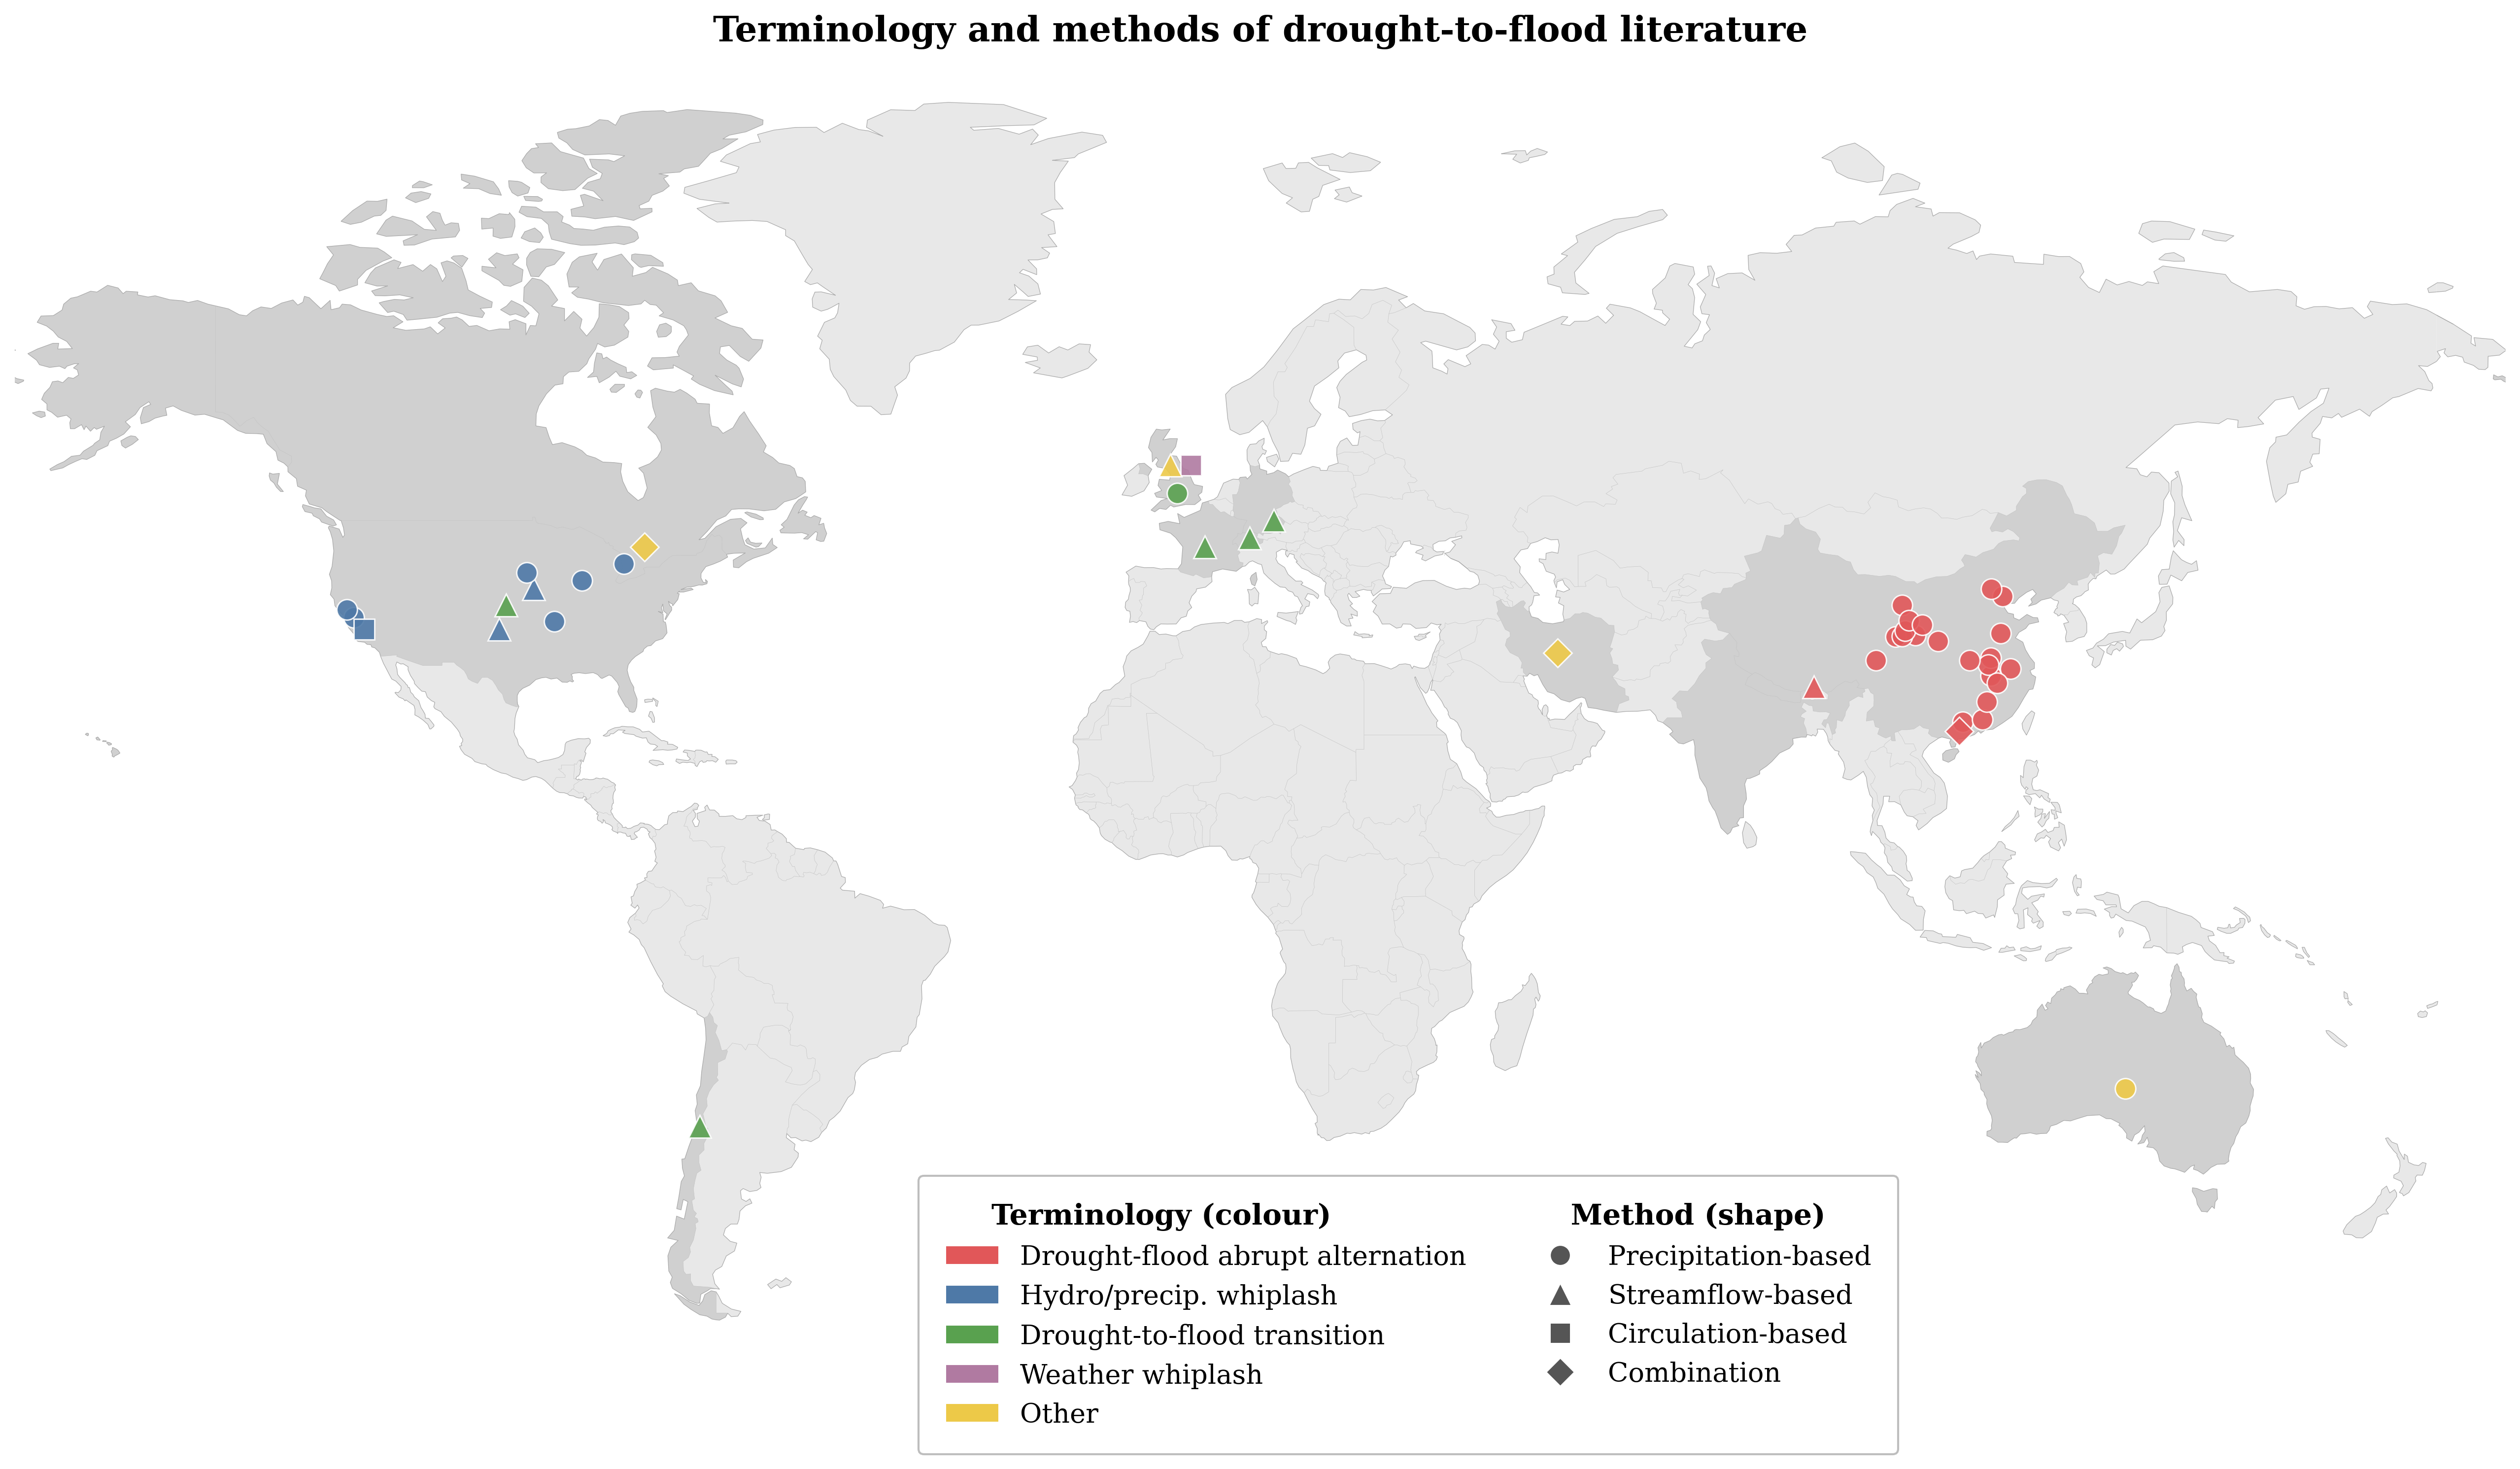
\includegraphics[width=\textwidth]
                {terminology_map.png}
        \end{column}

        \begin{column}{0.23\textwidth}
            \centering
            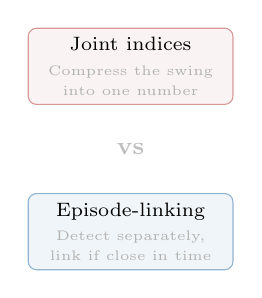
\begin{tikzpicture}[
                vs/.style={font=\small\bfseries, text=gray!50}
            ]

            % Joint indices (red — matches China cluster)
            \node[draw=gapred!50, rounded corners=3pt,
                  minimum width=2.6cm, minimum height=0.9cm,
                  fill=gapred!6, align=center, font=\scriptsize] (ji) at (0, 1.2)
                {Joint indices\\[0.1em]
                 {\tiny\color{gray!60} Compress the swing}\\[-0.1em]
                 {\tiny\color{gray!60} into one number}};

            \node[vs] at (0, 0.15) {vs};

            % Episode-linking (blue — matches US/Europe)
            \node[draw=vennblue!60, rounded corners=3pt,
                  minimum width=2.6cm, minimum height=0.9cm,
                  fill=vennblue!8, align=center, font=\scriptsize] (el) at (0, -0.9)
                {Episode-linking\\[0.1em]
                 {\tiny\color{gray!60} Detect separately,}\\[-0.1em]
                 {\tiny\color{gray!60} link if close in time}};

            \end{tikzpicture}
        \end{column}

    \end{columns}

\end{frame}

% --------------------------------------------------
% BACKUP: Research traditions comparison
% --------------------------------------------------
% USE: If panel asks "what does the literature look
%      like?", "how fragmented is the field?", or
%      follows the terminology map slide.
% --------------------------------------------------
\begin{frame}{Three research traditions}

    \centering
    \vspace{-0.3em}

    \footnotesize
    \renewcommand{\arraystretch}{1.4}
    \begin{tabular}{l l l l}
    \toprule
     & \textbf{DFAA} & \textbf{Western whiplash / transition} & \textbf{Weather whiplash} \\
    \midrule
    Origin          & Chinese hydrology          & US and Europe                          & Atmospheric science \\
    Primary variable & Precipitation (SPI-based)  & Precipitation, streamflow, or both     & 500\,hPa geopotential height \\
    Detection logic  & Purpose-built alternation   & Independent episode detection,         & Regime classification \\
                     & indices (single scalar)     & linked by temporal proximity           & via self-organising maps \\
    Seasonality      & Monsoon-specific            & Various                                & Synoptic timescales \\
    Research focus   & Characterisation            & Trends and prediction                  & Regime dynamics \\
    Role of ML       & None                        & Emerging                               & None \\
    \bottomrule
    \end{tabular}

    \vspace{0.8em}
    \scriptsize
    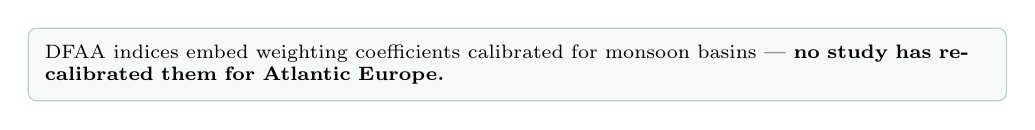
\begin{tikzpicture}
        \node[draw=ucdgreen!30, rounded corners=3pt, fill=ucdgreen!4,
              text width=12cm, align=left, font=\scriptsize, inner sep=6pt] {
            DFAA indices embed weighting coefficients calibrated for monsoon basins ---
            \textbf{no study has recalibrated them for Atlantic Europe.}
        };
    \end{tikzpicture}

\end{frame}

% --------------------------------------------------
% BACKUP: Three detection strategies
% --------------------------------------------------
% USE: If panel asks "how will you detect events?",
%      "what's the difference between thresholding and indices?"
% --------------------------------------------------
\definecolor{strat1}{RGB}{78, 121, 167}   % steel blue
\definecolor{strat2}{RGB}{225, 87, 89}    % warm red
\definecolor{strat3}{RGB}{176, 122, 161}  % muted purple

\tikzset{
    detbox/.style={draw=#1!70, thick, rounded corners=3pt,
                fill=#1!8, minimum width=3.0cm, minimum height=0.7cm,
                align=center, font=\scriptsize},
    detdata/.style={draw=gray!50, thick, rounded corners=3pt,
                fill=gray!6, minimum width=3.2cm, minimum height=0.7cm,
                align=center, font=\scriptsize},
    detresult/.style={draw=#1!70, thick, rounded corners=3pt,
                fill=#1!15, minimum width=3.2cm, minimum height=0.7cm,
                align=center, font=\scriptsize\bfseries},
    detarr/.style={-{Stealth[length=2mm]}, thick, #1!60},
    detlbl/.style={font=\footnotesize\bfseries, text=#1},
}

\begin{frame}{Three strategies for detecting transitions}

    \centering
    \vspace{-0.3em}

    \begin{tikzpicture}[xshift=0.5cm]

    % === Column 1: Raw thresholding ===
    \node[detlbl=strat1] (t1) at (1.0, 3.8) {1. Raw thresholding};
    \node[detdata] (d1) at (1.0, 3.0) {Streamflow};
    \node[detbox=strat1] (th1) at (1.0, 1.8) {Threshold directly\\(e.g.\ $<$Q20, $>$Q90)};
    \node[detbox=strat1] (link1) at (1.0, 0.6) {Link drought + flood\\episodes by proximity};
    \node[detresult=strat1] (ev1) at (1.0, -0.6) {DTF events};

    \draw[detarr=strat1] (d1) -- (th1);
    \draw[detarr=strat1] (th1) -- (link1);
    \draw[detarr=strat1] (link1) -- (ev1);

    \node[font=\tiny, text=gray, anchor=north, text width=3cm, align=center]
        at (1.0, -1.15) {Anderson (2025), G\"otte \&\\Brunner (2024), Yang (2025),\\Matan\'o (2024)};

    % === Column 2: Index-based thresholding ===
    \node[detlbl=strat2] (t2) at (5.5, 3.8) {2. Index-based};
    \node[detdata] (d2) at (5.5, 3.0) {Precipitation};
    \node[detbox=strat2] (idx) at (5.5, 1.8) {Compute index\\(SPI, SPEI, LDFAI, etc.)};
    \node[detbox=strat2] (th2) at (5.5, 0.6) {Threshold the index\\to identify events};
    \node[detresult=strat2] (ev2) at (5.5, -0.6) {DTF events};

    \draw[detarr=strat2] (d2) -- (idx);
    \draw[detarr=strat2] (idx) -- (th2);
    \draw[detarr=strat2] (th2) -- (ev2);

    \node[font=\tiny, text=gray, anchor=north, text width=3cm, align=center]
        at (5.5, -1.15) {Wang (2024), Bai (2024),\\Zhao (2024)};

    % === Column 3: Regime classification ===
    \node[detlbl=strat3] (t3) at (10.5, 3.8) {3. Regime classification};
    \node[detdata] (d3) at (10.5, 3.0) {500\,hPa height\\anomalies};
    \node[detbox=strat3] (som) at (10.5, 1.8) {Cluster circulation\\patterns};
    \node[detbox=strat3] (shift) at (10.5, 0.6) {Identify regime\\shifts};
    \node[detresult=strat3] (ev3) at (10.5, -0.6) {DTF events};

    \draw[detarr=strat3] (d3) -- (som);
    \draw[detarr=strat3] (som) -- (shift);
    \draw[detarr=strat3] (shift) -- (ev3);

    \node[font=\tiny, text=gray, anchor=north, text width=3cm, align=center]
        at (10.5, -1.15) {Francis et al.\ 2023};

    % === Caution annotation ===
    \node[draw=gapred!40, rounded corners=3pt, fill=gapred!4,
          text width=12cm, align=left, font=\scriptsize, inner sep=6pt]
        at (5.25, -2.6) {
            Yang et al.\ (2025) applied methods 1 and 2 to 7 decades of US catchment data and found \textbf{opposite frequency trends}.
        };

    \end{tikzpicture}

\end{frame}

% --------------------------------------------------
% BACKUP: Event definition choices across studies
% --------------------------------------------------
% USE: If panel asks "what thresholds will you use?",
%      "how are these events actually defined?", or
%      "what did other studies find?"
% --------------------------------------------------
\begin{frame}{How are drought-to-flood events defined?}

    \centering
    \vspace{-0.5em}

    \scriptsize
    \renewcommand{\arraystretch}{1.25}
    \begin{tabular}{l l c l l l}
    \toprule
    \textbf{Study} & \textbf{Region} & \textbf{Strategy} & \textbf{Drought def.} & \textbf{Flood def.} & \textbf{Transition rule} \\
    \midrule
    G\"otte \&      & US      & 1 & Streamflow $<$ Q20       & Streamflow $>$ Q50       & $\geq$10 days \\
    Brunner (2024)  &         &   & (varies by day-of-year)  & of annual maxima         & \\
    \arrayrulecolor{gray!30}\midrule\arrayrulecolor{black}
    Yang et         & US      & 1 & Streamflow $<$ Q50       & Streamflow $>$ Q50       & $<$90 days \\
    al.\ (2025)     &         &   & of annual 7-day min      & of annual maxima         & \\
    \arrayrulecolor{gray!30}\midrule\arrayrulecolor{black}
    Matan\'o et     & Global  & 1 & $<$Q15 in $\geq$1        & Streamflow               & $<$30 days \\
    al.\ (2024)     &         &   & hydrological variable    & $>$ Q85                  & \\
    \arrayrulecolor{gray!30}\midrule\arrayrulecolor{black}
    Guimar\~aes     & France  & 1 & Streamflow $<$ Q20       & Streamflow $>$ Q99       & No gap \\
    et al.\ (2026)  &         &   &                          &                          & \\
    \arrayrulecolor{gray!30}\midrule\arrayrulecolor{black}
    Wang et         & China   & 2 & SPI $\to$ MSDFAI         & SPI $\to$ MSDFAI         & Index $\geq$ 1 \\
    al.\ (2024)     &         &   & (alternation index)      & (alternation index)      & \\
    \bottomrule
    \end{tabular}

    \vspace{0.8em}
    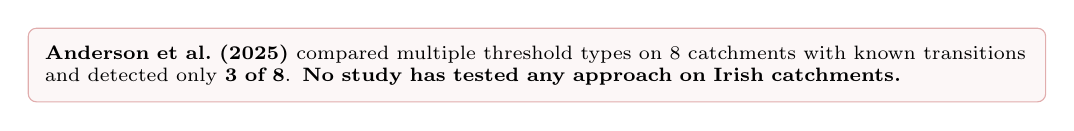
\begin{tikzpicture}
        \node[draw=gapred!40, rounded corners=3pt, fill=gapred!4,
              text width=12.5cm, align=left, font=\scriptsize, inner sep=6pt] {
            \textbf{Anderson et al.\ (2025)} compared multiple threshold types on 8~catchments
            with known transitions and detected only \textbf{3 of 8}.
            \textbf{No study has tested any approach on Irish catchments.}
        };
    \end{tikzpicture}

\end{frame}

% --------------------------------------------------
% BACKUP: Verification metrics
% --------------------------------------------------
% USE: If panel asks about the specific metrics used,
%      or wants to see the ACC equation.
% --------------------------------------------------
\begin{frame}{Verification Metrics}

    \vspace{-0.3em}

    {\footnotesize
    $f_i$ = forecast weekly mean, \quad
    $o_i$ = observed weekly mean, \quad
    $\bar{c}_i$ = climatological mean (1991--2020) \\[0.3em]
    $f'_i = f_i - \bar{c}_i$ = forecast anomaly, \quad
    $o'_i = o_i - \bar{c}_i$ = observed anomaly, \quad
    $N$ = number of cases
    }

    \vspace{0.5em}

    \begin{columns}[T]
    \begin{column}{0.48\textwidth}
        \[
        \mathrm{Bias} = \frac{1}{N}\sum_{i=1}^{N} (f_i - o_i)
        \]

        \[
        \mathrm{RMSE} = \sqrt{\frac{1}{N}\sum_{i=1}^{N} (f_i - o_i)^2}
        \]
    \end{column}

    \begin{column}{0.48\textwidth}
        \[
        \mathrm{ACC} = \frac{\displaystyle\sum_{i} f'_i \, o'_i}
        {\sqrt{\displaystyle\sum_{i} (f'_i)^2} \;\sqrt{\displaystyle\sum_{i} (o'_i)^2}}
        \]

        \vspace{0.3em}
        {\scriptsize
        Uncentred, unweighted, matching the ECMWF operational definition.
        Computed as spatial pattern correlation per init (across gridpoints),
        then averaged across inits.}
    \end{column}
    \end{columns}

\end{frame}

% --------------------------------------------------
% BACKUP: Variables in the pipeline
% --------------------------------------------------
% USE: If panel asks "what exactly is being verified?"
%      or "why those specific variables?"
%
% Processing verified against DECISIONS.md temporal resolution table:
%   t2m:  forecasts 6h inst → daily mean (4 values).
%         ERA5-Land hourly → 6h subset → daily mean (4 values).
%         Met Éireann hourly → daily mean (24 values).
%   tp:   forecasts 6h accum → de-accum → daily total (4 intervals).
%         ERA5-Land hourly accum → de-accum → daily total (24 hours).
%         Met Éireann daily total (native).
%   u10/v10: forecasts 6h inst. ERA5-Land hourly → 6h subset. (intermediate only)
%   ws10: derived sqrt(u10²+v10²) at 6h, then daily mean. Met Éireann hourly → daily mean.
% --------------------------------------------------
\begin{frame}{Pipeline Variables}

    \centering

    \footnotesize
    \renewcommand{\arraystretch}{1.4}
    \begin{tabular}{l l l l l l}
    \toprule
    \textbf{Var.} & \textbf{Seasonal} & \textbf{Subseasonal} & \textbf{ERA5-Land} & \textbf{Met \'Eireann} & \textbf{Verif.\ res.} \\
    \midrule
    t2m  & Daily mean      & Daily mean      & Daily mean        & Daily mean    & Daily \\
         & (from 6h inst.) & (from 6h inst.) & (from 6h subset)  & (from hourly) & \\[0.4em]
    tp   & Daily total     & Daily total     & Daily total       & Daily total   & Daily \\
         & (de-accum.\ 6h) & (de-accum.\ 6h) & (from hourly)    & (native)      & \\[0.4em]
    ws10 & Daily mean      & Daily mean      & Daily mean        & Daily mean    & Daily \\
         & (from 6h u10, v10) & (from 6h u10, v10) & (from 6h u10, v10) & (from hourly) & \\
    \bottomrule
    \end{tabular}

    \vspace{1em}
    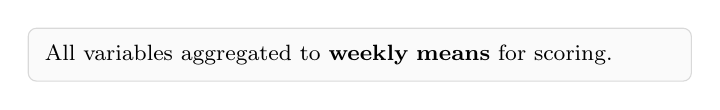
\begin{tikzpicture}
        \node[draw=gray!30, rounded corners=3pt, fill=gray!4,
              text width=8cm, align=left, font=\footnotesize, inner sep=6pt] {
            All variables aggregated to \textbf{weekly means} for scoring.
        };
    \end{tikzpicture}

\end{frame}

% --------------------------------------------------
% BACKUP: Station-level deterministic verification
% --------------------------------------------------
% USE: If panel asks "show me a specific station",
%      "how does skill decay with lead time?", or
%      "which forecast variant is best?"
% --------------------------------------------------
\begin{frame}{Station-Level Verification}

    \begin{columns}[c, totalwidth=\textwidth]

        \begin{column}{\textwidth}
            \centering
            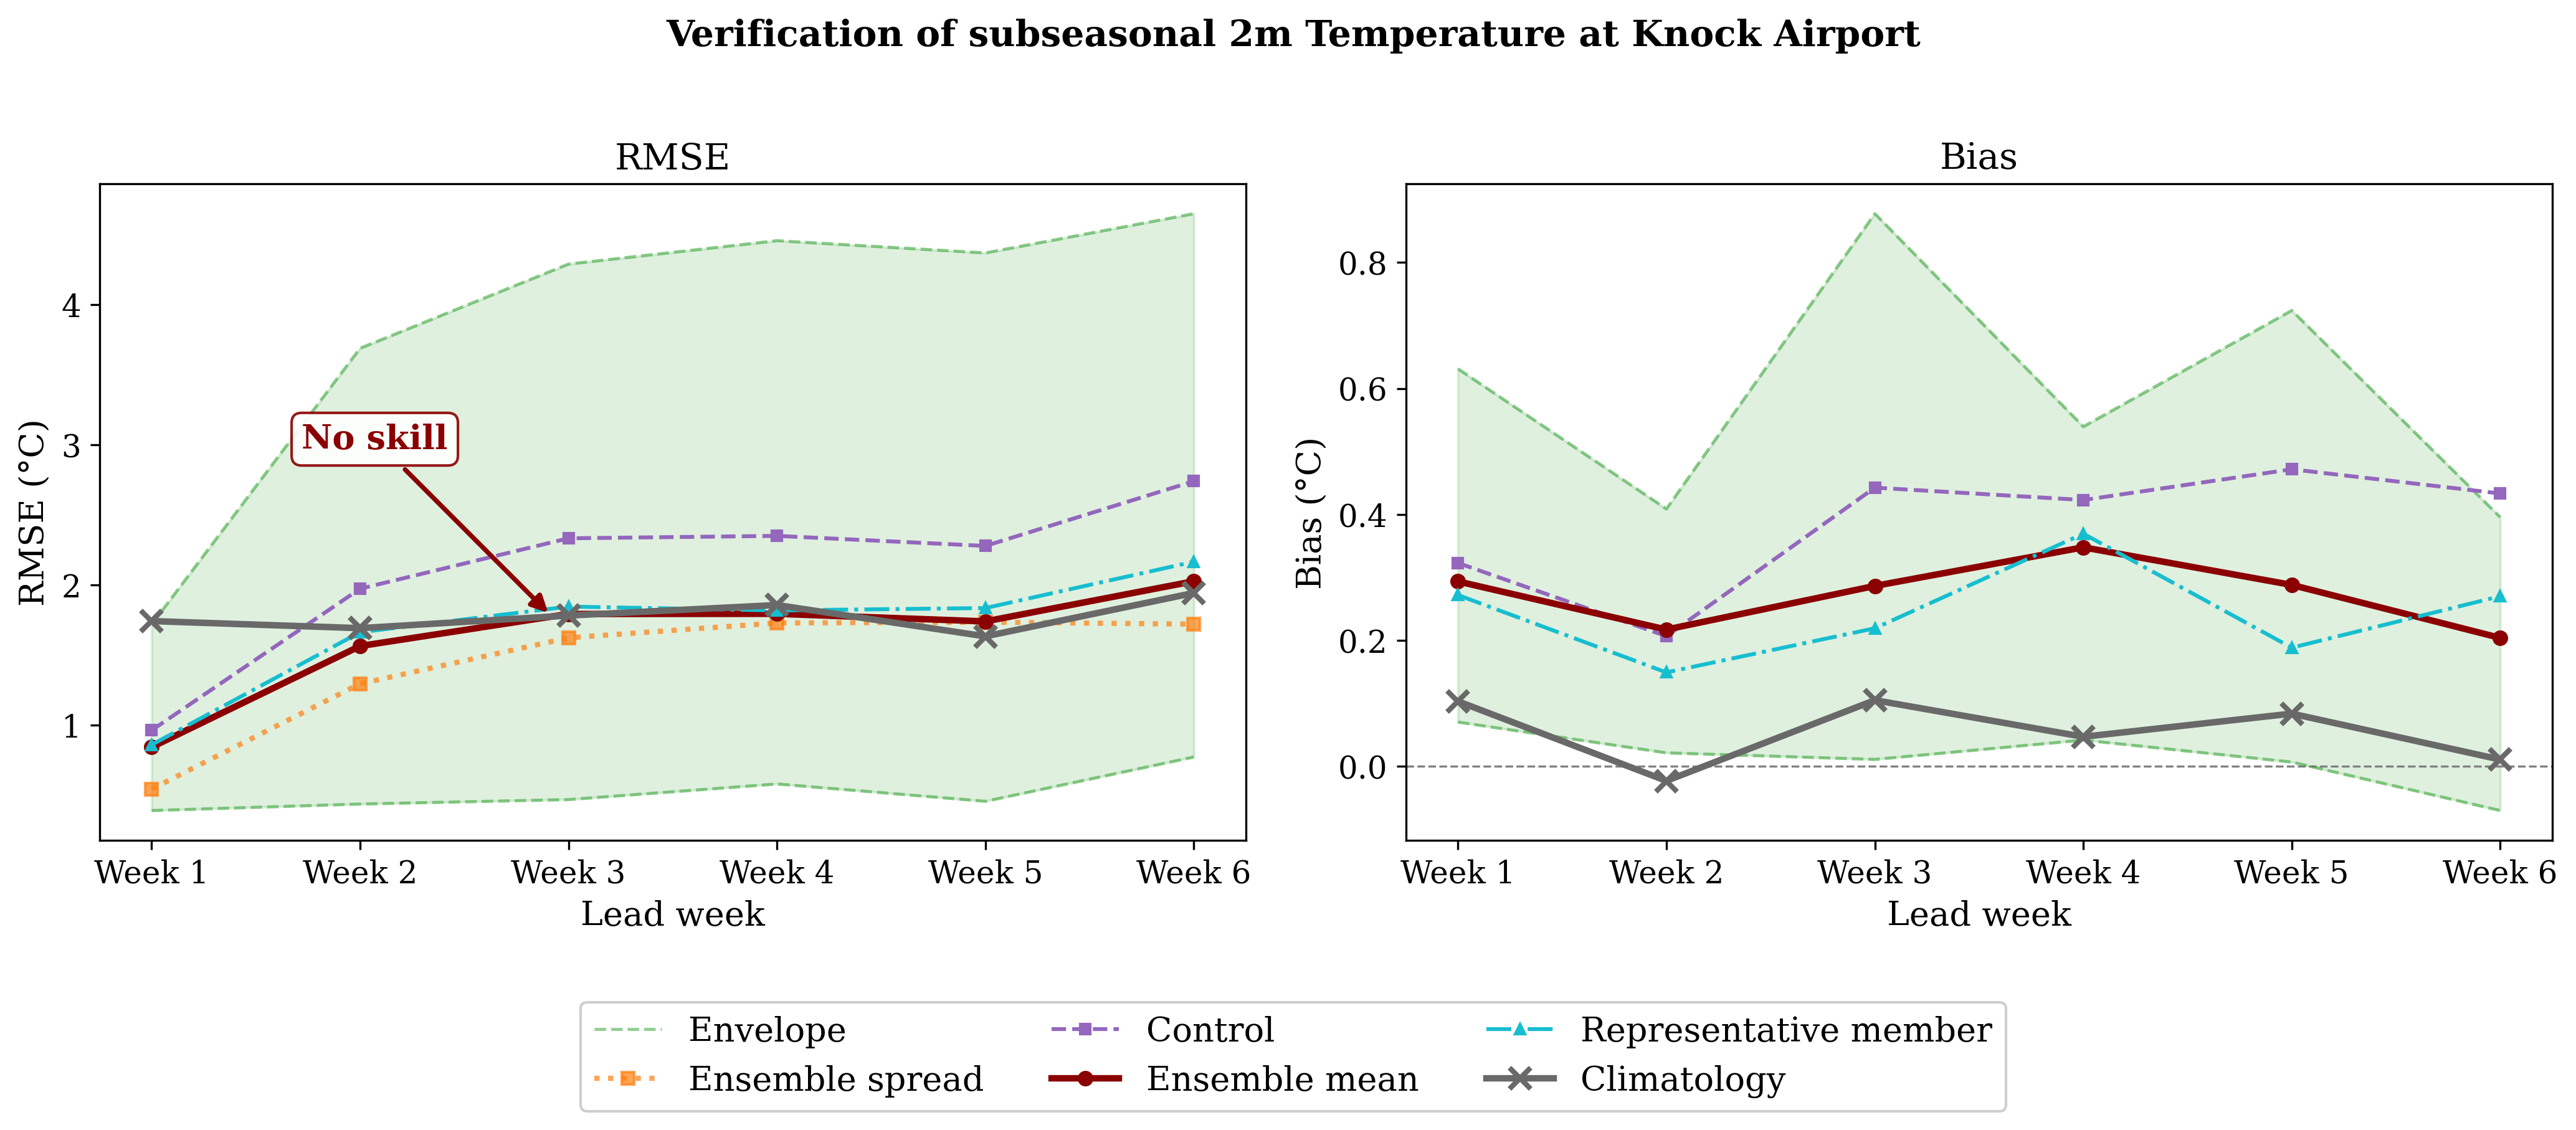
\includegraphics[width=\textwidth, height=0.80\textheight, keepaspectratio]{slide_rmse_bias_t2m_hly4935.png}
        \end{column}

    \end{columns}

\end{frame}

% --------------------------------------------------
% BACKUP: Spatial RMSE
% --------------------------------------------------
% USE: If panel asks about spatial error magnitude,
%      or wants to see RMSE maps alongside bias.
% --------------------------------------------------
\begin{frame}{Spatial RMSE}

    \begin{columns}[c, totalwidth=\textwidth]

        \begin{column}{\textwidth}
            \centering
            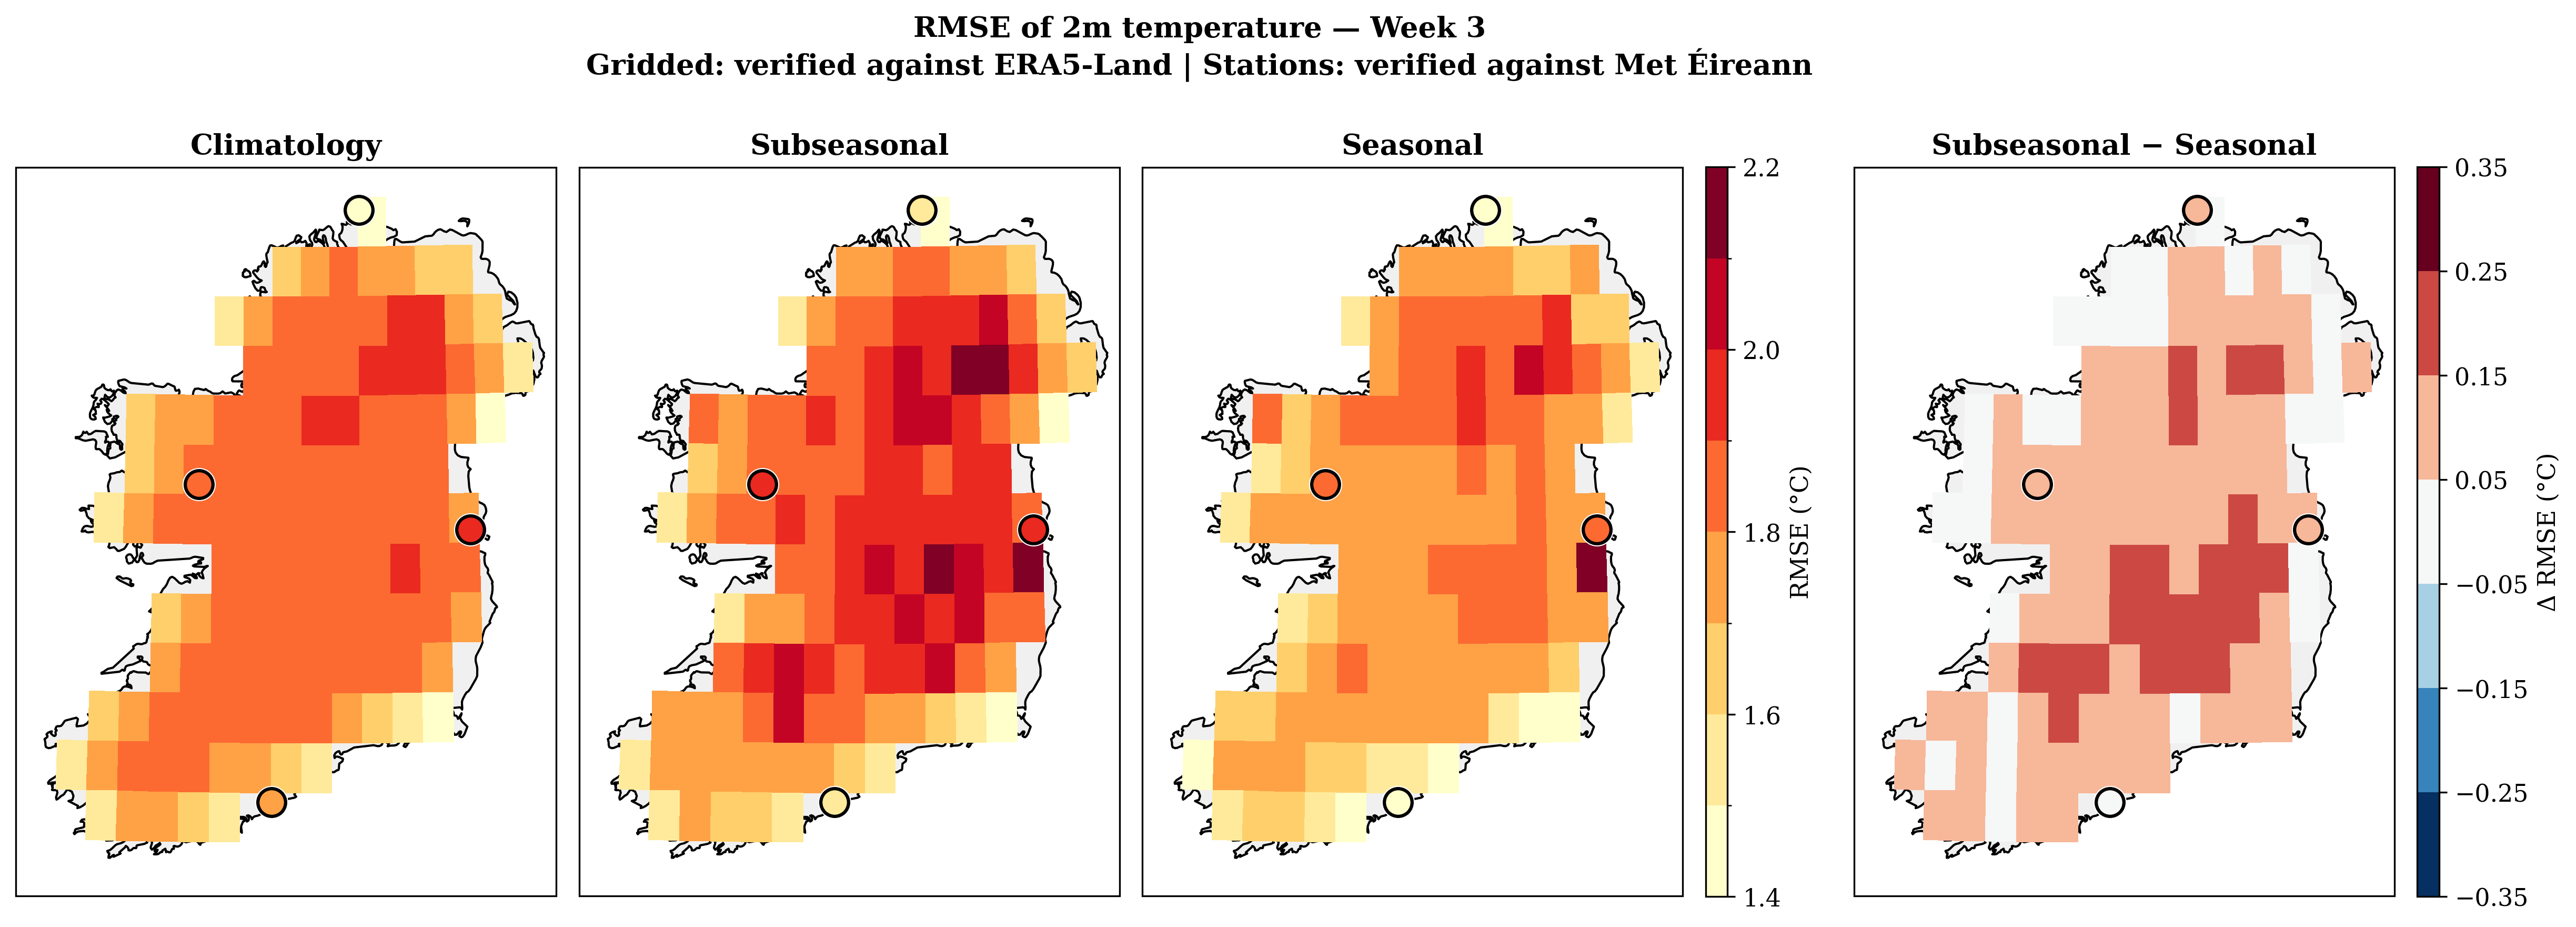
\includegraphics[width=\textwidth, height=0.85\textheight, keepaspectratio]{consolidation_spatial_rmse_4panel.png}
        \end{column}

    \end{columns}

\end{frame}

% --------------------------------------------------
% BACKUP: Spatial Skill Score (RMSS)
% --------------------------------------------------
% USE: If panel asks "does the forecast beat climatology?"
%      or "where is there actual skill?"
% --------------------------------------------------
\begin{frame}{Spatial Skill Score}

    \vspace{-0.5em}
    \begin{columns}[c, totalwidth=\textwidth]

        \begin{column}{0.72\textwidth}
            \centering
            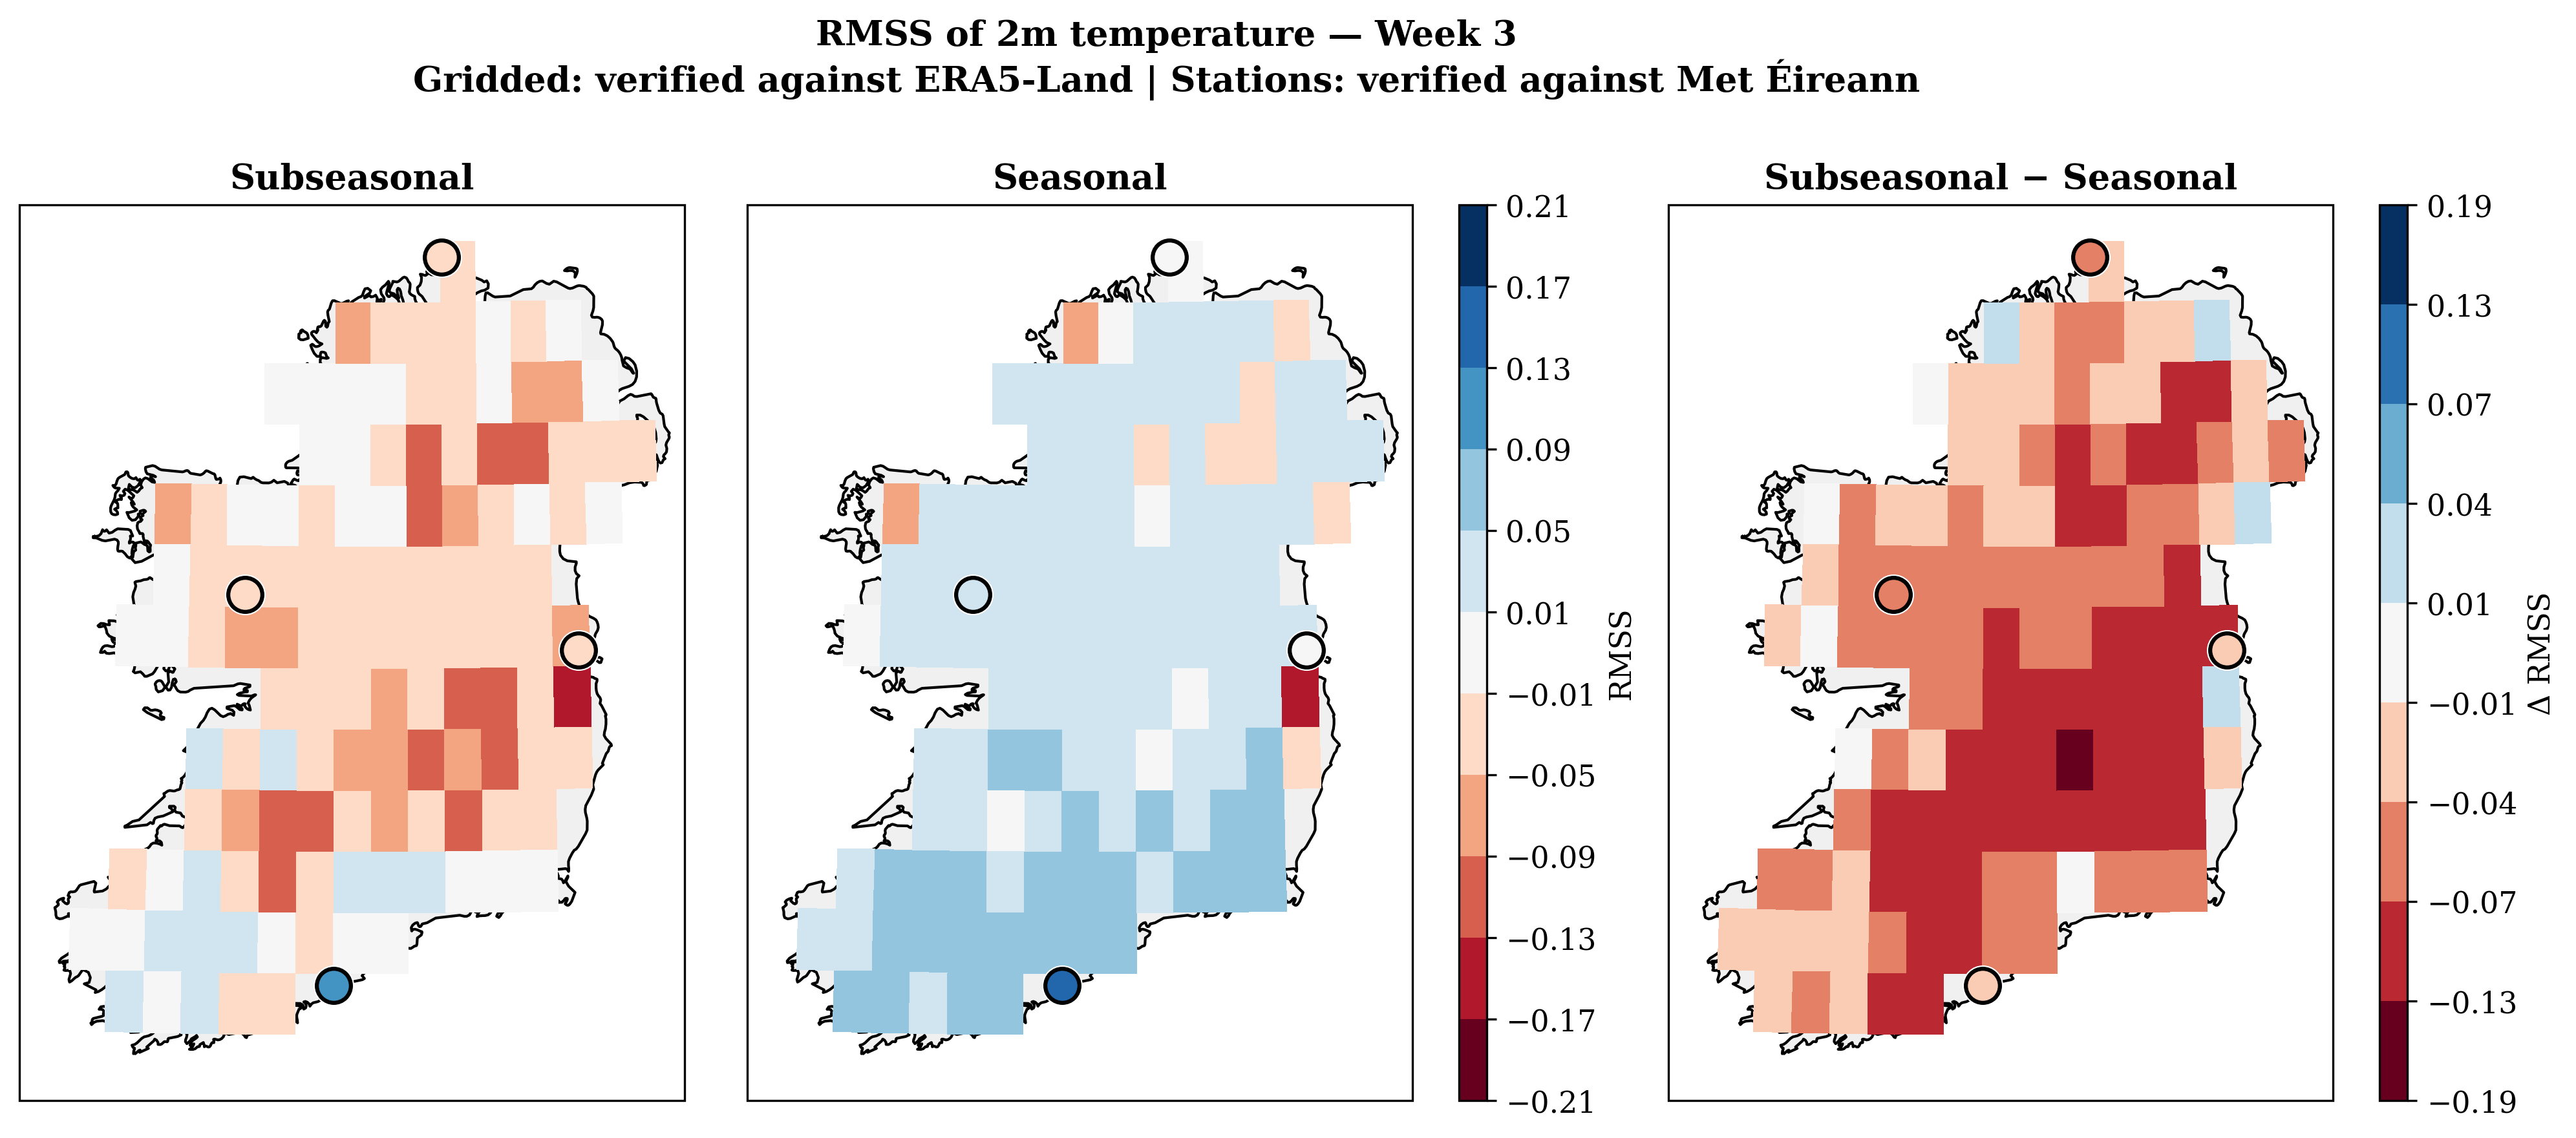
\includegraphics[width=\textwidth, height=0.80\textheight, keepaspectratio]{consolidation_spatial_rmss_3panel.png}
        \end{column}

        \begin{column}{0.26\textwidth}
            \vspace{1em}
            \begin{block}{\small RMSS}
            \small
            \[
                \text{RMSS} = 1 - \frac{\text{RMSE}_{\text{fc}}}{\text{RMSE}_{\text{clim}}}
            \]
            \vspace{0.3em}

            \textbf{RMSS $> 0$}: forecast beats climatology\\[0.3em]
            \textbf{RMSS $= 0$}: no skill\\[0.3em]
            \textbf{RMSS $< 0$}: worse than climatology
            \end{block}
        \end{column}

    \end{columns}

\end{frame}

% --------------------------------------------------
% BACKUP: Literature review scope (Venn diagram)
% --------------------------------------------------
% USE: If panel asks "how did you scope the review?"
%      or "what fields does this draw from?"
% --------------------------------------------------
\begin{frame}{Where the Literature Review Sits}

    \centering
    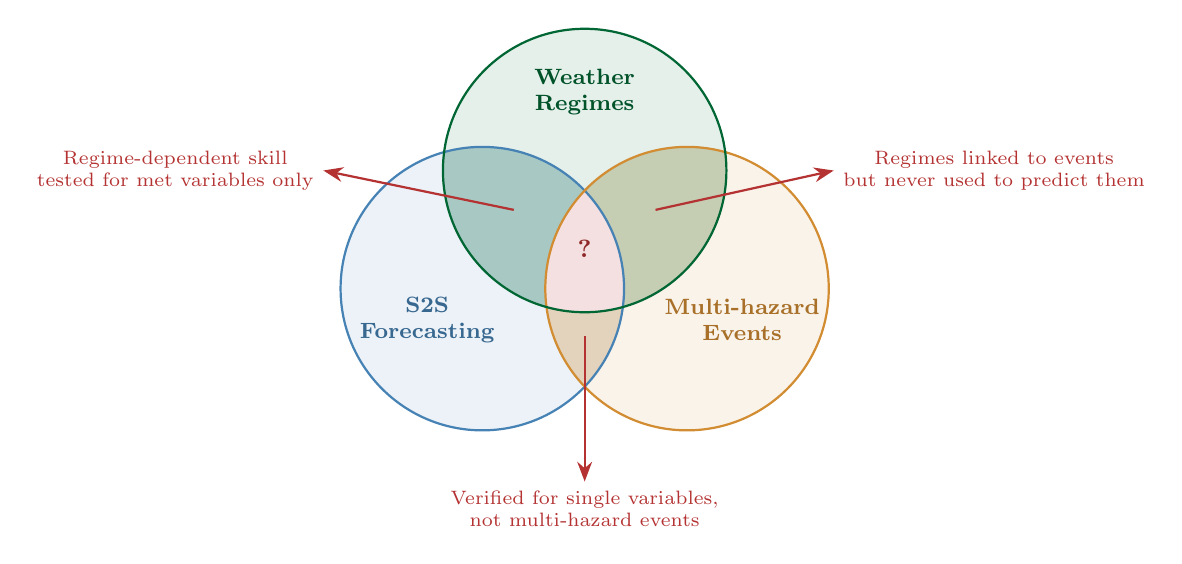
\begin{tikzpicture}
    \def\r{1.8}

    % Base circle fills
    \fill[vennblue!10] (-1.3,0) circle (\r);
    \fill[vennorange!10] ( 1.3,0) circle (\r);
    \fill[ucdgreen!10] (0,1.5) circle (\r);

    % Pairwise overlap fills
    \begin{scope}
      \clip (-1.3,0) circle (\r);
      \clip ( 1.3,0) circle (\r);
      \fill[vennblue!25!vennorange, opacity=0.3] (-3,-3) rectangle (3,3);
    \end{scope}
    \begin{scope}
      \clip (-1.3,0) circle (\r);
      \clip (0,1.5) circle (\r);
      \fill[vennblue!40!ucdgreen, opacity=0.3] (-3,-3) rectangle (3,3);
    \end{scope}
    \begin{scope}
      \clip ( 1.3,0) circle (\r);
      \clip (0,1.5) circle (\r);
      \fill[ucdgreen!40!vennorange, opacity=0.3] (-3,-3) rectangle (3,3);
    \end{scope}

    % Triple intersection fill
    \begin{scope}
      \clip (-1.3,0) circle (\r);
      \clip ( 1.3,0) circle (\r);
      \clip (0,1.5) circle (\r);
      \fill[gapred!15] (-3,-3) rectangle (3,3);
    \end{scope}

    % Circle outlines
    \draw[vennblue, thick] (-1.3,0) circle (\r);
    \draw[vennorange, thick] ( 1.3,0) circle (\r);
    \draw[ucdgreen, thick] (0,1.5) circle (\r);

    % Circle labels
    \node[align=center, text=vennblue!80!black, font=\footnotesize\bfseries]
        at (-2.0,-0.4) {S2S\\Forecasting};
    \node[align=center, text=vennorange!80!black, font=\footnotesize\bfseries]
        at ( 2.0,-0.4) {Multi-hazard\\Events};
    \node[align=center, text=ucdgreen!80!black, font=\footnotesize\bfseries]
        at (0,2.5) {Weather\\Regimes};

    % Centre — the thesis
    \node[align=center, font=\small\bfseries, text=gapred!80!black]
        at (0,0.5) {?};

    % Pairwise gap labels
    % S2S × Multi-hazard (bottom)
    \node[align=center, font=\scriptsize, text=gapred] (g1) at (0,-2.8)
         {Verified for single variables,\\not multi-hazard events};
    \draw[-{Stealth[length=2.5mm]}, thick, gapred] (0,-0.6) -- (g1.north);

    % S2S × Weather Regimes (upper-left)
    \node[align=center, font=\scriptsize, text=gapred] (g2) at (-5.2,1.5)
         {Regime-dependent skill\\tested for met variables only};
    \draw[-{Stealth[length=2.5mm]}, thick, gapred] (-0.9,1.0) -- (g2.east);

    % Weather Regimes × Multi-hazard (upper-right)
    \node[align=center, font=\scriptsize, text=gapred] (g3) at (5.2,1.5)
         {Regimes linked to events\\but never used to predict them};
    \draw[-{Stealth[length=2.5mm]}, thick, gapred] (0.9,1.0) -- (g3.west);

    \end{tikzpicture}

\end{frame}

% --------------------------------------------------
% BACKUP: Variable availability matrix
% --------------------------------------------------
% USE: If panel asks "what variables are available?"
%      or "why only three variables?"
% --------------------------------------------------
\begin{frame}{Variable Availability}

    \centering

    % TikZ matrix for variable availability
    \newcommand{\cw}{0.6}   % cell width in cm
    \newcommand{\ch}{0.5}   % cell height in cm
    \begin{tikzpicture}[
        cell/.style={minimum width=\cw cm, minimum height=\ch cm, inner sep=0pt, outer sep=0pt},
        avail/.style={cell, fill=availgreen!80},
        deriv/.style={cell, fill=derivblue!60},
        noavail/.style={cell, fill=unavailgray!40},
        partial/.style={cell, fill=partialgreen!30},
        hdr/.style={font=\tiny\bfseries, rotate=55, anchor=south west},
        rowlbl/.style={font=\footnotesize, anchor=east},
        brace/.style={decorate, decoration={calligraphic brace, amplitude=4pt, raise=2pt},
                      thick, ucdgreen!60},
    ]

    % Category grouping braces — all categories get braces for consistency
    \draw[brace] (0*\cw, 3.1) -- node[above=6pt, font=\tiny\color{gray}] {Temperature} (3*\cw, 3.1);
    \draw[brace] (3*\cw, 3.1) -- node[above=6pt, font=\tiny\color{gray}] {Precip.} (4*\cw, 3.1);
    \draw[brace] (4*\cw, 3.1) -- node[above=6pt, font=\tiny\color{gray}] {Wind} (7*\cw, 3.1);
    \draw[brace] (7*\cw, 3.1) -- node[above=6pt, font=\tiny\color{gray}] {Humid.} (8*\cw, 3.1);
    \draw[brace] (8*\cw, 3.1) -- node[above=6pt, font=\tiny\color{gray}] {Radiation} (12*\cw, 3.1);
    \draw[brace] (12*\cw, 3.1) -- node[above=6pt, font=\tiny\color{gray}] {Heat flux} (14*\cw, 3.1);
    \draw[brace] (14*\cw, 3.1) -- node[above=6pt, font=\tiny\color{gray}] {Pressure} (16*\cw, 3.1);
    \draw[brace] (16*\cw, 3.1) -- node[above=6pt, font=\tiny\color{gray}] {Cloud} (18*\cw, 3.1);
    \draw[brace] (18*\cw, 3.1) -- node[above=6pt, font=\tiny\color{gray}] {Other} (20*\cw, 3.1);

    % Column headers — positioned tight above grid
    \def\cols{t2m/0, tmax/1, tmin/2, tp/3, u10/4, v10/5, ws10/6, d2m/7, ssrd/8, strd/9, ssr/10, str/11, slhf/12, sshf/13, msl/14, sp/15, tcc/16, sun/17, snow/18, evap/19}

    \foreach \name/\col in \cols {
        \node[hdr] at (\col*\cw+0.08, 2.3) {\name};
    }

    % Row labels
    \node[rowlbl] at (-0.2, 2.0) {Seasonal};
    \node[rowlbl] at (-0.2, 1.45) {Subseasonal};
    \node[rowlbl] at (-0.2, 0.9) {ERA5-Land};
    \node[rowlbl] at (-0.2, 0.35) {Met \'Eireann};

    % --- Seasonal row ---
    \foreach \col/\s in {0/avail, 1/avail, 2/avail, 3/avail, 4/avail, 5/avail, 6/deriv, 7/avail, 8/avail, 9/avail, 10/avail, 11/avail, 12/avail, 13/avail, 14/avail, 15/avail, 16/avail, 17/avail, 18/avail, 19/avail} {
        \node[\s] at (\col*\cw+\cw/2, 2.0) {};
    }

    % --- Subseasonal row ---
    \foreach \col/\s in {0/avail, 1/avail, 2/avail, 3/avail, 4/avail, 5/avail, 6/deriv, 7/avail, 8/avail, 9/avail, 10/avail, 11/avail, 12/avail, 13/avail, 14/avail, 15/avail, 16/avail, 17/noavail, 18/avail, 19/noavail} {
        \node[\s] at (\col*\cw+\cw/2, 1.45) {};
    }

    % --- ERA5-Land row ---
    \foreach \col/\s in {0/avail, 1/deriv, 2/deriv, 3/avail, 4/avail, 5/avail, 6/deriv, 7/avail, 8/avail, 9/avail, 10/avail, 11/avail, 12/avail, 13/avail, 14/deriv, 15/avail, 16/noavail, 17/noavail, 18/avail, 19/avail} {
        \node[\s] at (\col*\cw+\cw/2, 0.9) {};
    }

    % --- Met Éireann row ---
    \foreach \col/\s in {0/avail, 1/deriv, 2/deriv, 3/avail, 4/noavail, 5/noavail, 6/avail, 7/avail, 8/noavail, 9/noavail, 10/noavail, 11/noavail, 12/noavail, 13/noavail, 14/avail, 15/noavail, 16/partial, 17/partial, 18/noavail, 19/noavail} {
        \node[\s] at (\col*\cw+\cw/2, 0.35) {};
    }

    % Grid lines
    \foreach \row in {0.35, 0.9, 1.45, 2.0} {
        \foreach \col in {0,...,19} {
            \draw[gray!20] (\col*\cw, \row-\ch/2) rectangle +(\cw, \ch);
        }
    }

    % Legend — below plot
    \node[font=\scriptsize, anchor=north] at (6, -0.3) {%
        \begin{tikzpicture}[baseline=-0.5ex]
            \fill[availgreen!80] (0,0) rectangle (0.25,0.25);
            \node[right, font=\scriptsize] at (0.35,0.125) {Available};
            \fill[derivblue!60] (2.3,0) rectangle (2.55,0.25);
            \node[right, font=\scriptsize] at (2.65,0.125) {Derivable};
            \fill[unavailgray!40] (4.6,0) rectangle (4.85,0.25);
            \node[right, font=\scriptsize] at (4.95,0.125) {Not available};
            \fill[partialgreen!30] (7.4,0) rectangle (7.65,0.25);
            \node[right, font=\scriptsize] at (7.75,0.125) {Partial (12 synoptic)};
        \end{tikzpicture}%
    };

    \end{tikzpicture}

\end{frame}

\end{document}
